% !TEX root = ../axiomatic.tex

\section{Proof}\label{s:proof}

In this section we present the proof of our main theorem: any non-degenerate and irreducible \mbox{cup-$i$} construction is isomorphic to the canonical one.
We divide this proof into several parts.

In \cref{ss:properties} we recast the axioms defining our characterization in the language introduced in the previous section.
A useful consequence of freeness is recorded in \cref{ss:consequence}.
The base case of an induction argument is given in \cref{ss:cases}; whereas in
\cref{ss:fact} we recall a fact about our presentation of the canonical cup-$i$ construction.
We devote \cref{ss:preparing} to prepare an induction step and \cref{ss:step} to present it.
Our theorem is finally proven in \cref{ss:proof} using the foreshadowed induction argument.

\subsection{Axioms revisited}\label{ss:properties}

We start by recasting the axioms introduced in \cref{d:properties} using the reformulation of the previous section.
We then observe that the canonical cup-$i$ construction satisfies them.

\begin{lemma}\label{l:properties}
	Consider for each $i,n \in \N$ an indexing set $\Lambda(i,n)$ and an element
	\[
	\triangle_i [n] =
	\sum_{\mathclap{\lambda \in \Lambda(i,n)}} V_\lambda \ot W_\lambda
	\]
	in $\cP(\simplex^n)^{\ot 2}_{i+n}$ with each $V_\lambda \ot W_\lambda$ in its basis.
	Assume $\triangle = \big\{ \triangle_i [n] \big\}_{i,n \in \N}$ defines a \mbox{cup-$i$} construction, then:
	\begin{enumerate}
		\item $\triangle$ is non-degenerate iff
		$\triangle_0 [0] = \emptyset \ot \emptyset$.
		\item $\triangle$ is irreducible iff\,
		$\forall i,n \in \N$, $\forall \lambda \in \Lambda(i,n)$, $V_\lambda \cap W_\lambda = \emptyset$.
	\end{enumerate}
\end{lemma}

\begin{proof}
	By naturality, it suffices to verify these equivalences for the \mbox{cup-$i$} product structure defined on $\cochains(X)$ when $X = \simplex^n$ for every $n \in \N$.
	We will use the fact that the isomorphism $\Psi_n^{\ot 2} \colon \cP(\gsimplex^n)^{\ot 2} \to \chains(\gsimplex^n)^{\ot 2}$ sends basis elements to basis elements, as does the linear duality isomorphism between chains and cochains.

	\noindent (1) This follows from the fact that $\chains(\gsimplex^0)^{\ot 2}$ is 1-dimensional and generated by $[0] \ot [0] = \Psi_0^{\ot 2} (\emptyset \ot \emptyset)$.
	Explicitly, if $x$ is a $0$-simplex with dual basis element denoted $x^\vee$, the only two options for $x^\vee \cup_0 x^\vee$ are $x^\vee$ or $0$, with the first holding if and only if $\triangle_0[0] = \emptyset \ot \emptyset$.

	\noindent (2) To prove this equivalence notice that there is $k \in V_\lambda \cap W_\lambda$ for one of the summands of $\triangle_i [n]$ if an only the image of this summand under $\Psi_n^{\ot 2}$ is
	\[
	\underbrace{d_{V_\lambda \setminus k} \overbrace{d_k[n]}^{y}}_{y^{(1)}}
	\ot
	\underbrace{d_{W_\lambda \setminus k} \overbrace{d_k[n]}^{y}}_{y^{(2)}}
	\]
	with $y^{(1)} \smallsmile_i y^{(2)} \neq 0$.
\end{proof}

The following is deduced from \cref{l:properties} by inspecting \cref{l:canonical}.

\begin{theorem}\label{t:existence}
	The canonical \mbox{cup-$i$} construction is non-degenerate and irreducible.
\end{theorem}

\subsection{irreducible chains}

A basis element $V \ot W \in \cP(\simplex^n)^{\ot 2}$ is said to be \textit{irreducible} if $V \cap W = \emptyset$ and \textit{reducible} otherwise.
Let $\pired \colon \cP(\simplex^n)^{\ot 2} \to \cP(\simplex^n)^{\ot 2}$ be the projection to the subspace generated by reducible basis elements.
Explicitly,
\[
\pired(V \ot W) =
\begin{cases}
	V \ot W, & \text{if $V \ot W$ is reducible},\\
	\hfil 0, & \text{if not}.
\end{cases}
\]
A chain $\zeta \in \cP(\simplex^n)^{\ot 2}$ is said to be \textit{irreducible} if $\pired(\zeta) = 0$.
%or \textit{strongly reducible} if $\pired(\zeta) = \zeta$.
Notice that, by \cref{l:properties}, a cup-$i$ construction $\triangle$ is irreducible if and only if $\triangle_i[n]$ is irreducible
%\[
%\pired(\triangle_i[n]) = 0
%\]
for all $i, n \in \N$.

\subsection{Partition chains}

For any $U \subseteq \set{0,\dots,n}$, its \textit{partition chain} $\zeta_U$ to be the sum of all irreducible basis elements $V \ot W$ with $V \union W = U$ and $V \cap W = \emptyset$.

\begin{lemma}\label{l:partition chains}
	An irreducible chain $\zeta \in \cP(\simplex^n)^{\ot 2}$ satisfies $(\pired \circ \bd)(\zeta) = 0$ iff $\zeta$ is a sum of partition chains.
\end{lemma}

\begin{proof}
	Consider an irreducible chain $\zeta = \sum_{\Lambda} V \ot W$ with $\Lambda$ a subset of the basis of $\cP(\simplex^n)^{\ot 2}$.
	Its boundary can be decomposed as follows
	\[
	\bd \zeta = \sum_{\Lambda} \Big(\sum_{w \in W} w.V \ot W \ + \ \sum_{v \in V} V \ot v.W \ +
	\sum_{\bar u \notin V \union W} \bar u.V \ot  W + V \ot \bar u.W\Big).
	\]
	Therefore,
	\[
	(\pired \circ \bd) \zeta = \sum_{\Lambda} \Big(\sum_{w \in W} w.V \ot W \ + \ \sum_{v \in V} V \ot v.W\Big).
	\]
	Let us consider two irreducible basis elements $V \ot W$ and $V' \ot W'$, and elements $v \in V$, $w \in W$, $v' \in V'$, and $w' \in W'$.
	The following simple implications hold by direct inspection
	\begin{align*}
		&(w.V \ot W = w'.V' \ot W') &\implies& &&(w = w') \wedge (V = V') \wedge (W = W'), \\
		&(V \ot v.W = V' \ot v'.W') &\implies& &&(v = v') \wedge (V = V') \wedge (W = W'), \\
		&(w.V \ot W = V' \ot v'.W') &\implies& &&(w = v') \wedge (V' = w.V) \wedge (W' = W \setminus v'), \\
		&(V \ot v.W = w'.V' \ot W') &\implies& &&(v = w') \wedge (V' = V \setminus w) \wedge (W' = v.W).
	\end{align*}
	Now, if $(\pired \circ \bd) \zeta = 0$, these imply that for $V \ot W \in \Lambda$, $v \in V$, and $w \in W$ both $w.V \ot W \setminus w \in \Lambda$ and $V \setminus v \ot v.W \in \Lambda$.
	From this it follows that $\Lambda$ contains all irreducible basis elements $V' \ot W'$ with $V' \union W' = V \ot W$, that is to say, all summands of the partition chain of $V \union W$.
	Conversely, the above also implies that $(\pired \circ \bd)\zeta_U = 0$ for any partition chain $\zeta_U$.
	\anibal{Maybe write more about this direction.}
\end{proof}

\subsection{Special cases}\label{ss:cases}

\anibal{Is the only degenerate construction the 0 construction?}

We relate cup-$i$ constructions satisfying some of our axioms to the canonical cup-$i$ construction for special values of $i,n \in \N$.
These will serve as the base case of an induction argument in \cref{ss:proof}.

\begin{lemma}\label{l:special case one}
	Let $\big\{ \triangle_i [n] \big\}_{i,n\in\N}$ be free and non-degenerate \mbox{cup-$i$} construction and, as always, let $\big\{ \Delta_i [n] \big\}_{i,n\in\N}$ be the canonical one.
	\begin{enumerate}
		\item \label{i:i>n} $\forall i,n \in \N$, $\triangle_i[n] = \Delta_i [n] = 0$ if $i > n$.
		\item \label{i:i=n} $\forall n \in \N$, $\triangle_n[n] = \Delta_n [n] = \emptyset \ot \emptyset$.
	\end{enumerate}
\end{lemma}

\begin{proof}
	The chain complex $\cP(\simplex^n)^{\ot 2}$ is $0$ in degrees greater than $2n$ and it is generated by $\emptyset \ot \emptyset$ in degree $2n$.

	The claim in \cref{i:i>n} is immediate since $\triangle_i[n]$ is in degree $n+i > 2n$ if $i > n$.

	If the conclusion of the claim in \cref{i:i=n} does not hold, there exists $n \in \N$ smallest such that $\triangle_n [n] = 0$.
	If $n > 0$ then
	\begin{align*}
	(1+T) \triangle_{n-1} [n] =
	\bd \triangle_{n} [n] + \triangle_{n} \bd \, [n] = 0,
	\end{align*}
	and \cref{l:consequence} implies $\triangle_{n-1} [n] = 0$.
	From this and the assumption
	\[
	\triangle_{n-1}[n-1] = \emptyset \ot \emptyset
	\]
	we obtain
	\begin{equation}
	\begin{split}
	(1+T)\triangle_{n-2} [n] =
	\bd \triangle_{n-1} [n] + \triangle_{n-1} \bd \, [n] =
	\sum_{u = 0}^n \{u\} \ot \{u\},
	\end{split}
	\end{equation}
	which is a contradiction since $\sum_u \{u\} \ot \{u\}$ is not in the image of $(1+T)$.

	The previous argument shows that $\triangle_n [n] = 0$ for every $n \in \N$.
	This serves as the base case of an induction argument over $n-i$ that will prove $\triangle_i [n] = 0$ for every $i, n \in \N$; a contradiction to the non-degeneracy of the cup-$i$ construction.
	For the induction step, consider
	\begin{align*}
	(1+T) \triangle_{i-1} [n] =
	\bd \triangle_{i} [n] + \triangle_{i} \bd\, [n] = 0,
	\end{align*}
	which, by \cref{l:consequence}, implies $\triangle_{i-1} [n] = 0$.
\end{proof}

\begin{lemma}\label{l:special case two}
	Let $\big\{ \triangle_i [n] \big\}_{i,n\in\N}$ be free and non-degenerate \mbox{cup-$i$} construction.
	For all integer $n \geq 1$ either $\triangle_{n-1} [n]$ or $T \triangle_{n-1} [n]$ is equal to
	\[
	\Delta_{n-1} [n] \defeq
	\sum_{\mathclap{\substack{u \in \{0,\dots,n\} \\ u \ \mathrm{odd}}}} \{u\} \ot \emptyset +
	\sum_{\mathclap{\substack{u \in \{0,\dots,n\} \\ u \ \mathrm{even}}}} \emptyset \ot \{u\}.
	\]
\end{lemma}

\begin{proof}
	By \cref{l:special case one} we have $\triangle_{n} [n] = \emptyset \ot \emptyset$ and $\triangle_{n} \bd \, [n] = 0$ for all $n \in \N$.
	Therefore,
	\begin{align*}
	(1+T) \triangle_{n-1} [n] &=
	(\bd \ot \, \id + \id \ot \bd) (\emptyset \ot \emptyset) \\ &=
	(1+T) \sum_{u=0}^n \{u\} \ot \emptyset
	\end{align*}
	and we need to show that the partition of the indexing set $\{0, \dots, n\} = \Lambda_0 \sqcup \Lambda_1$ provided by \cref{l:consequence} is determined by the parity of integers.
	Let us argue by contradiction assuming some $j$ and $j+1$ belong to the same $\Lambda_{\varepsilon}$.
	With no loss of generality let us assume $\varepsilon = 0$ so we have
	\[
	\triangle_{n-1} [n] = \big( \{j\} + \{j+1\} \big) \ot \emptyset + O(j, j+1)
	\]
	where $O(j, j+1)$ is a sum of basis elements missing $\{j\}$ and $\{j+1\}$ from both of its tensor factors.
	Since $\triangle_{n-1} \bd \, [n] = \sum_{u=0}^{n} \{u\} \ot \{u\}$,
	\[
	(1+T) \triangle_{n-2} [n] = (1+T) \big( \{j\} \ot \{j+1\} \big) + P(j, j+1)
	\]
	where $P(j, j+1)$ is a sum of basis elements with $j$ and $j+1$ missing from at least one of its tensor factors.

	By \cref{l:kernel of sxs} every basis element in $P(j,j+1)$ is in the $\ker \cP(\sigma_j)^{\ot 2}$.
	Using \cref{l:consequence} in the above equation implies that $\triangle_{n-2}[n]$, an element in $\ker \cP(\sigma_j)^{\ot 2}$, is equal to either $\big( \{j\} \ot \{j+1\} \big)$ or $\big( \{j+1\} \ot \{j\} \big)$ plus an element in this kernel.
	This is a contradiction since neither of these two basis elements is in $\ker \cP(\sigma_j)^{\ot 2}$ by \cref{l:kernel of sxs}.
\end{proof}

\subsection{Facts about our formulas}\label{ss:fact}

We reprint two statements proven in \cite{medina2023fast_sq}.

\begin{notation*}
	For $U \in \P_{n-i}^n$ we write $\bar u \notin U$ if $\bar u \in \{0, \dots, n\} \setminus U$.
	We simplify notation writing $\bar u.U$ instead of $\{\bar u\} \union U$ if $\bar u \notin U$ and $U \setminus u$ instead of $U \setminus \{u\}$ if $u \in U$.
\end{notation*}

\begin{proposition}[{\cite[Lemma~21]{medina2023fast_sq}}]\label{p:fact1}
	For $i,n \in \N$ with $i < n$ we have:
	\[
	\Delta_i \bd \, [n] =
	\sum_{\mathclap{U \in \P_{n-i}^n}} \
	\left(\
	\sum_{\mathclap{u \in U^1}} u.U^0 \ot U^1 +
	\sum_{\mathclap{u \in U^0}} U^0 \ot u.U^1
	\right).
	\]
\end{proposition}

\begin{proposition}[{\cite[Lemma~??]{medina2023fast_sq}}]\label{p:fact2}
	TBW
\end{proposition}

\subsection{Preparing the induction step}\label{ss:preparing}

We will prove two statements that are key to prove the induction step of the argument establishing our main result.

\begin{notation*}
	Given a function $\xi \colon \P_{n-i}^n \to \F$ we denote by $\barxi \colon \P_{n-i}^n \to \F$ the function defined by the condition $\barxi(U) \neq \xi(U) \text{ for all } U \in \P_{n-i}^n$.
	We will simplify notation writing $U^\xi$ and $U^{\barxi}$ instead of $U^{\xi(U)}$ and $U^{\barxi(U)}$.
\end{notation*}

%\begin{lemma}\label{l:first nail}
%	Let $\big\{ \triangle_i [n] \big\}_{i,n\in\N}$ be a free and non-degenerate \mbox{cup-$i$} construction and $i,n \in \N$ with $i \leq n-2$.
%	If there is a function $\xi \colon \P_{n-i}^n \to \F$ with
%	\begin{equation}\label{e:xi and barxi}
%	\triangle_i [n] =
%	\sum_{\mathclap{U \in \P_{n-i}^n}} U^{\xi} \ot U^{\barxi}
%	\end{equation}
%	then the following implications hold:
%	\begin{alignat*}{2}
%		&\boxed{\triangle_i [n-1] = \Delta_i [n-1] \kern 7.3pt}\ &\Longrightarrow\
%		&\boxed{\triangle_i [n] = \Delta_i [n] \kern 7.3pt} \\
%		&\boxed{\triangle_i [n-1] = T \Delta_i [n-1]}\ &\Longrightarrow\
%		&\boxed{\triangle_i [n] = T \Delta_i [n]} \ .
%	\end{alignat*}
%\end{lemma}
%
%\begin{proof}
%	Let us assume $\triangle_i [n-1] = \Delta_i [n-1]$.
%	The other case is proven analogously.
%	Applying the boundary of $\cP(\simplex^n)^{\ot 2}$ -- \cref{e:boundary of P} -- to \cref{e:xi and barxi} gives
%	\begin{align*}
%	\bd \triangle_i [n] & =
%	\sum_{\mathclap{U \in \P_{n-i}^n}} \
%	\left(\
%	\sum_{\mathclap{\bar u \notin U}} \bar u.U^\xi \ot U^\barxi +
%	\sum_{\mathclap{\bar u \notin U}} U^\xi \ot \bar u.U^\barxi
%	\right) \\ & +
%	\sum_{\mathclap{U \in \P_{n-i}^n}} \
%	\left(\
%	\sum_{\mathclap{u \in U^\barxi}} u.U^\xi \ot U^\barxi +
%	\sum_{\mathclap{u \in U^{\xi}}} U^\xi \ot u.U^\barxi
%	\right).
%	\end{align*}
%	Combining our assumption and \cref{p:fact1} gives
%	\[
%	\triangle_i \bd \, [n] =
%	\Delta_i \bd \, [n] =
%	\sum_{\mathclap{U \in \P_{n-i}^n}} \
%	\left(\
%	\sum_{\mathclap{u \in U^1}} u.U^0 \ot U^1 +
%	\sum_{\mathclap{u \in U^0}} U^0 \ot u.U^1
%	\right).
%	\]
%	Adding this last two identities together gives
%	\[
%	(1+T) \triangle_{i-1} [n] =
%	\bd \triangle_i [n] + \triangle_i \bd \, [n] =
%	S_1 + S_2
%	\]
%	where
%	\[
%	S_1 = \sum_{\mathclap{U \in \P_{n-i}^n}} \
%	\left(\
%	\sum_{\mathclap{\bar u \notin U}} \bar u.U^\xi \ot U^\barxi +
%	\sum_{\mathclap{\bar u \notin U}} U^\xi \ot \bar u.U^\barxi
%	\right)
%	\]
%	and
%	\[
%	S_2 = (1+T) \sum_{\mathclap{\substack{U \in \P_{n-i}^n \\ \xi(U) \neq 0}}} \
%	\left(\
%	\sum_{\mathclap{u \in U^1}} u.U^0 \ot U^1 +
%	\sum_{\mathclap{u \in U^0}} U^0 \ot u.U^1
%	\right).
%	\]
%	A summand $V \ot W$ is said to be irreducible if $V \cap W = \emptyset$ and reducible otherwise.
%	We notice that all the summands in $S_1$ are irreducible whereas all in $S_2$ are not.
%	Therefore, if $S_2$ is not $0$, there is a reducible element in $\triangle_{i-1}[n]$ which is a contradiction.
%	We will see that the only way for $S_2$ to be $0$ is if $\xi(U) = 0$ for all $U \in \P_{n-i}^n$.
%	If two distinct summands are equal, the union of its tensor factors must agree, say $U \in \P_{n-i}^n$.
%	Additionally, their intersections, $u \in U$, do as well.
%	This implies that either
%	\[
%	u.U^0 \ot U^1 = U^1 \ot u.U^0 \quad \text{or} \quad
%	u.U^1 \ot U^0 = U^0 \ot u.U^1.
%	\]
%	In both cases, since $U^0 \cap U^1 = \emptyset$, we have that the cardinality of $U$ must be $1$, that is $n-i = 1$, which is a contradiction.
%	We have then that $\xi = 0$ is constant and therefore
%	\[
%	\triangle_i [n] =
%	\sum_{\mathclap{U \in \P_{n-i}^n}} U^0 \ot U^1
%	\]
%	as claimed.
%\end{proof}

\begin{lemma}\label{l:first nail}
	Let $\triangle = \set[\big]{\triangle_i[n]}_{i,n\in\N}$ be an irreducible and non-degenerate \mbox{cup-$i$} construction and $i,n \in \N$ with $i \leq n-2$.
	If there is a function $\xi \colon \P_{n-i}^n \to \F$ with
	\begin{equation}\label{e:xi and barxi}
		\triangle_i [n] =
		\sum_{\mathclap{U \in \P_{n-i}^n}} U^{\xi} \ot U^{\barxi} + \Phi
	\end{equation}
	where $\Phi \in \ker(1+T)$,	\anibal{and should not be summands of the form $U^0 \ot U^1$} then the following implications hold:
	\begin{alignat*}{2}
		&\boxed{\triangle_i [n-1] = \Delta_i [n-1] \kern 7.3pt}\ &\Longrightarrow\
		&\boxed{\triangle_i [n] = \Delta_i [n] \kern 7.3pt} \\
		&\boxed{\triangle_i [n-1] = T \Delta_i [n-1]}\ &\Longrightarrow\
		&\boxed{\triangle_i [n] = T \Delta_i [n]} \ .
	\end{alignat*}
	\anibal{Notice that each basis element in $\Phi$ must be in the kernel of $\P(\Sigma_j)$ for each $j$.}
\end{lemma}

\begin{proof}
	Let us assume $\triangle_i [n-1] = \Delta_i [n-1]$.
	The other case is proven analogously.
	Applying the boundary of $\cP(\simplex^n)^{\ot 2}$ -- \cref{e:boundary of P} -- to \cref{e:xi and barxi} gives
	\begin{align*}
		\bd \triangle_i [n] + \bd \Phi& =
		\sum_{\mathclap{U \in \P_{n-i}^n}} \
		\left(\
		\sum_{\mathclap{\bar u \notin U}} \bar u.U^\xi \ot U^\barxi +
		\sum_{\mathclap{\bar u \notin U}} U^\xi \ot \bar u.U^\barxi
		\right) \\ & +
		\sum_{\mathclap{U \in \P_{n-i}^n}} \
		\left(\
		\sum_{\mathclap{u \in U^\barxi}} u.U^\xi \ot U^\barxi +
		\sum_{\mathclap{u \in U^{\xi}}} U^\xi \ot u.U^\barxi
		\right).
	\end{align*}
	Combining our assumption and \cref{p:fact1} gives
	\[
	\triangle_i \bd \, [n] =
	\Delta_i \bd \, [n] =
	\sum_{\mathclap{U \in \P_{n-i}^n}} \
	\left(\
	\sum_{\mathclap{u \in U^1}} u.U^0 \ot U^1 +
	\sum_{\mathclap{u \in U^0}} U^0 \ot u.U^1
	\right).
	\]
	Adding this last two identities together gives
	\[
	(1+T) \triangle_{i-1} [n] =
	\bd \triangle_i [n] + \triangle_i \bd \, [n] =
	S_1 + S_2 + \bd \Phi
	\]
	where
	\[
	S_1 = \sum_{\mathclap{U \in \P_{n-i}^n}} \
	\left(\
	\sum_{\mathclap{\bar u \notin U}} \bar u.U^\xi \ot U^\barxi +
	\sum_{\mathclap{\bar u \notin U}} U^\xi \ot \bar u.U^\barxi
	\right)
	\]
	and
	\[
	S_2 = (1+T) \sum_{\mathclap{\substack{U \in \P_{n-i}^n \\ \xi(U) \neq 0}}} \
	\left(\
	\sum_{\mathclap{u \in U^1}} u.U^0 \ot U^1 +
	\sum_{\mathclap{u \in U^0}} U^0 \ot u.U^1
	\right).
	\]

	Since $\triangle$ is assumed irreducible, writing $\Phi$ in the canonical basis gives
	\[
	\Phi = (1+T)\sum_{\lambda\in\Lambda} V_\lambda \ot W_\lambda
	\]
	with $V_\lambda \cap W_\lambda = \emptyset$ for each $\lambda$ in $\Lambda$, and, by \cref{e:boundary of P},
	\[
	\bd\Phi = \sum_{\lambda\in\Lambda}
	\left(\
	\sum_{\mathclap{\bar v \notin V_\lambda}} \bar v.V_\lambda \ot W_\lambda +
	\sum_{\mathclap{\bar w \notin W_\lambda}} V_\lambda \ot \bar w.W_\lambda
	\right).
	\]

	A basis element $V \ot W$ is said to be \textit{irreducible} if $V \cap W = \emptyset$ and \textit{reducible} otherwise.
	We notice that all summands in $S_1$ are irreducible whereas all in $S_2$ are not.

	We write $\bd\Phi$ as $S_3 + S_4$ with
	\[
	S_3 = (1+T)\sum_{\lambda\in\Lambda} \
	\sum_{\mathclap{\hspace*{20pt}\bar u \notin V_\lambda \union W_\lambda}} \bar u.V_\lambda \ot W_\lambda + V_\lambda \ot \bar u.W_\lambda,
	\]
	with each summand an irreducible basis element, and
	\[
	S_4 = (1+T)\sum_{\lambda\in\Lambda}
	\left(\
	\sum_{w \in W_\lambda} w.V_\lambda \ot W_\lambda \ + \
	\sum_{v \in V_\lambda} V_\lambda \ot v.W_\lambda
	\right),
	\]
	with each summand a reducible one.
	Therefore, if $S_2 + S_4$ is not $0$, there is a reducible basis element in $\triangle_{i-1}[n]$, which is a contradiction.

	We will first see that basis element appearing as a summand in $S_2$ also appears as a summand in $S_4$.
	If not, there is a pair of summands in $S_2$ each equal to the same basis element.
	In this case, the union and intersection of their tensor factors is the same, say respectively equal to $U \in \P_{n-i}^n$ and $u \in U$.
	For one such pair $u$ and $U$ there correspond two summands in $S_2$, which are related by $T$, so, depending on the index of $u$ in $U$, we have
	\[
	u.U^0 \ot U^1 = U^1 \ot u.U^0 \quad \text{or} \quad
	u.U^1 \ot U^0 = U^0 \ot u.U^1.
	\]
	In both cases, since $U^0 \cap U^1 = \emptyset$, we have that the cardinality of $U$ must be $1$, that is, $n-i = 1$, a contradiction.

	Now, if $S_2 \neq 0$, without loss of generality we can consider a basis element $u.U^0 \ot U^1$ appearing as a summand.
	The previous analysis shows that there is $\lambda \in \Lambda$ such that $u.U^0 \ot U^1$ is equal to one of the following:
	\begin{align*}
		&\text{a) } u.V_\lambda \ot W_\lambda, &\text{b) }& V_\lambda \ot u.W_\lambda, \\
		&\text{c) } u.W_\lambda \ot V_\lambda, &\text{d) }& W_\lambda \ot u.V_\lambda.
	\end{align*}
	We can see that a) implies $U^0 \ot U^1 = V_\lambda \ot W_\lambda$ and that c) implies $U^1 \ot U^0 = V_\lambda \ot W_\lambda$, each conclusion contradicting our assumption on $\Phi$.

	We have then that $\xi = 0$ is constant and therefore
	\[
	\triangle_i [n] =
	\sum_{\mathclap{U \in \P_{n-i}^n}} U^0 \ot U^1
	\]
	as claimed.
\end{proof}

%\begin{lemma}\label{l:second nail}
%	Let $\big\{ \triangle_i [n] \big\}_{i,n\in\N}$ be a non-degenerate, irreducible, and free \mbox{cup-$i$} construction and $i,n \in \N$ with $i \leq n-2$.
%	If $\triangle_i [n] = \Delta_i [n]$ or $\triangle_i [n] = T \Delta_i [n]$ then the following implications hold:
%	\begin{alignat*}{2}
%	&\boxed{\triangle_i [n-1] = \Delta_i [n-1] \kern 7.3pt}\ &\Longrightarrow\
%	&\boxed{\triangle_i [n] = \Delta_i [n] \kern 7.3pt} \\
%	&\boxed{\triangle_i [n-1] = T \Delta_i [n-1]}\ &\Longrightarrow\
%	&\boxed{\triangle_i [n] = T \Delta_i [n]} \ .
%	\end{alignat*}
%\end{lemma}
%
%\begin{proof}
%	We use the convention $\triangle_{-1} [n] = \Delta_{-1} [n] = 0$ for all $n \in \N$.
%	We will establish the first of the implications above using a proof by contradiction for which we assume $\triangle_i [n-1] = \Delta_i [n-1]$ and $\triangle_i [n] = T \Delta_i [n]$.
%	The second implication is proven analogously.
%	We have
%	\begin{align*}
%	(1+T) \triangle_{i-1}[n] &=
%	\bd \triangle_i [n] + \triangle_i \bd \, [n] \\ &=
%	\bd T \Delta_i [n] + \Delta_i \bd \, [n] \\ &=
%	T \bd \Delta_i [n] + \bd \Delta_i [n] + \bd \Delta_i [n] + \Delta_i \bd \, [n] \\ &=
%	(1+T) \bd \Delta_i [n] + (1+T) \Delta_{i-1} [n] \\ &=
%	(1+T) \Delta_i \bd \, [n] + (1+T) \Delta_{i-1} [n].
%	\end{align*}
%	Using \cref{p:fact1,l:canonical}, i.e.
%	\[
%	\begin{split}
%	\Delta_i \bd \, [n] &=
%	\sum_{\mathclap{U \in \P_{n-i}^n}} \
%	\left(\
%	\sum_{\mathclap{u \in U^1}} u.U^0 \ot U^1 +
%	\sum_{\mathclap{u \in U^0}} U^0 \ot u.U^1
%	\right), \\
%	\Delta_{i-1} [n] &=
%	\sum_{\mathclap{V \in \P_{n-i+1}^n}} V^0 \ot V^1,
%	\end{split}
%	\]
%	we have
%	\begin{align*}
%	(1+T) \triangle_{i-1}[n] &=
%	(1+T) \sum_{\mathclap{U \in \P_{n-i}^n}} \
%	\left(\
%	\sum_{\mathclap{u \in U^1}} u.U^0 \ot U^1 +
%	\sum_{\mathclap{u \in U^0}} U^0 \ot u.U^1
%	\right) \\ &+
%	(1+T) \sum_{\mathclap{V \in \P_{n-i+1}^n}} V^0 \ot V^1.
%	\end{align*}
%	By \cref{l:consequence} there are functions $\eta \colon \P_{n-i}^n \to \F$ and $\zeta \colon \P_{n-i+1}^n \to \F$ such that
%	\begin{align*}
%	\triangle_{i-1}[n] \ &=
%	\sum_{\mathclap{U \in \P_{n-i}^n}} \
%	\left(\
%	\sum_{\mathclap{u \in U^\bareta}} u.U^\eta \ot U^\bareta +
%	\sum_{\mathclap{u \in U^\eta}} U^\eta \ot u.U^\bareta
%	\right) \\ &+
%	\sum_{\mathclap{V \in \P_{n-i+1}^n}} V^\zeta \ot V^\barzeta.
%	\end{align*}
%	This contradicts the irreducibility of $\big\{ \triangle_i [n] \big\}_{i,n \in \N}$ as expressed in \cref{l:properties}.
%\end{proof}

\subsection{Induction step}\label{ss:step}

We prove the induction step of the argument proving our main result.

\begin{figure}
	\centering
	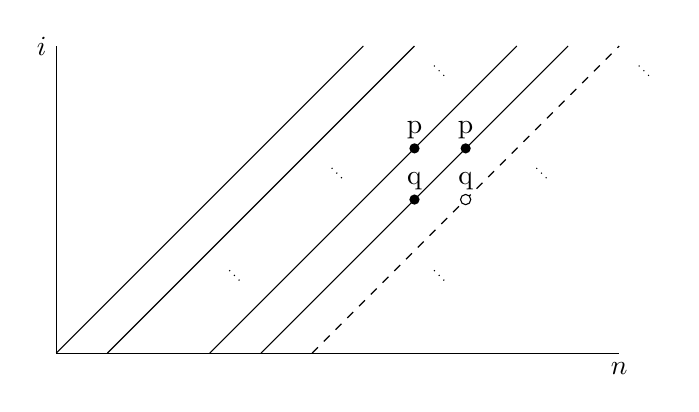
\begin{tikzpicture}[scale = .65]
	\draw (0,0)--(0,6);
	\draw (0,0)--(11,0);
	\draw (0,0)--(6,6);
	\draw (1,0)--(7,6);
	\draw (3,0)--(9,6);
	\draw (4,0)--(10,6);
	\draw[dashed] (5,0)--(11,6);

	\draw[dotted, shorten >=10pt,shorten <=10pt] (3,2)--(4,1);
	\draw[dotted, shorten >=10pt,shorten <=10pt] (5,4)--(6,3);
	\draw[dotted, shorten >=10pt,shorten <=10pt] (7,6)--(8,5);

	\fill (7,4) circle (0.1);
	\fill (8,4) circle (0.1);
	\fill (7,3) circle (0.1);
	\fill[white] (8,3) circle (0.1);
	\draw (8,3) circle (0.1);

	\node[above] at (7,4) {p};
	\node[above] at (8,4) {p};
	\node[above] at (7,3) {q};
	\node[above] at (8,3) {q};

	\draw[dotted, shorten >=10pt,shorten <=10pt] (7,2)--(8,1);
	\draw[dotted, shorten >=10pt,shorten <=10pt] (9,4)--(10,3);
	\draw[dotted, shorten >=10pt,shorten <=10pt] (11,6)--(12,5);

	\node[below] at (11,0) {$n$};
	\node[left] at (0,6) {$i$};
	\end{tikzpicture}
	\caption{Representation of the implication in \cref{l:induction step} serving as the induction step in the proof of \cref{t:main}.}
	\label{f:induction step}
\end{figure}

\begin{lemma}\label{l:induction step}
	Let $\set[\big]{\triangle_i [n]}_{i,n\in\N}$ be a free non-degenerate and irreducible \mbox{cup-$i$} construction.
	Let $\set[\big]{\p(i,n)}_{i,n \in \N}$ and $\set{\q(i,n)}_{i,n \in \N}$ each be one of the following two families of propositions:
	\[
	\big\{ \triangle_i [n] = \Delta_ i [n] \big\}_{i,n \in \N}
	\quad \text{or} \quad
	\big\{ \triangle_i [n] = T \Delta_ i [n] \big\}_{i,n \in \N} \ .
	\]
	For all $i,n \in \N$ with $i \leq n-2$ the following implication holds:
	\[
	\boxed{\p(i+1,n) \wedge \p(i+1,n-1) \wedge \q(i,n-1)}\ \Longrightarrow\ \boxed{\q(i,n)}
	\]
\end{lemma}

\begin{proof}
	Let both $\big\{ \p(i,n) \big\}_{i,n\in\N}$ and $\big\{ \q(i,n) \big\}_{i,n\in\N}$ be the family $\big\{ \triangle_i [n] = \Delta_i [n] \big\}_{i,n \in \N}$.
	The other three combinations are treated analogously.

	From $\p(i+1,n)$ and $\p(i+1,n-1)$ we have
	\[
	\bd \triangle_{i+1} [n] + \triangle_{i+1} \bd \, [n] =
	\bd \Delta_{i+1} [n] + \Delta_{i+1} \bd \, [n]
	\]
	or, equivalently,
	\begin{align*}
	(1+T) \triangle_i [n] =
	(1+T) \Delta_i [n] \defeq
	(1+T) \sum_{\mathclap{U \in \P_{n-i}^n}} {U^0} \ot {U^1}
	\end{align*}
	\cref{l:consequence} implies the existence of a function $\xi \colon \rP_{n-i}^n \to \Ftwo$ such that
	\[
	\triangle_i [n] =
	\sum_{\mathclap{U \in \P_{n-i}^n}} U^\xi \ot U^\barxi.
	\]
	\cref{l:first nail} implies, using $\q(i,n-1)$, that
	\[
	\triangle_i [n] = \Delta_i [n]
	\quad \text{or} \quad
	\triangle_i [n] = T \Delta_i [n].
	\]
	Finally, \cref{l:second nail} implies $\triangle_i [n] = \Delta_i [n]$, i.e., $\q(i,n)$.
\end{proof}

\subsection{Complete proof}\label{ss:proof}

We now present the proof of our main result.

\begin{proof}[Proof of \cref{t:main}]
	Let $\triangle = \set[\big]{\triangle_i [n]}_{i,n\in\N}$ be a non-degenerate and irreducible \mbox{cup-$i$} construction.
	Let $\set[\big]{\p(i,n)}_{i,n \in \N}$ and $\set{\q(i,n)}_{i,n \in \N}$ each be one of the following two families of propositions:
	\[
	\set[\big]{\triangle_i [n] = \Delta_ i [n]}_{i,n \in \N}
	\quad \text{or} \quad
	\set[\big]{\triangle_i [n] = T \Delta_ i [n]}_{i,n \in \N} \ .
	\]
	We need to show that for any fixed $i$ either $\p(i,n)$ or $\q(i,n)$ hold for every $n$.
	We will use an induction argument over $k = n-i$ to show this.
	For $k \leq 0$, i.e. $i \geq n$, the both $\p(i,n)$ and $\q(i,n)$ hold by \cref{l:special case one}, whereas for $k = 1$ one of them does by \cref{l:special case two}.
	Let us assume that our claim holds for values less than $k = n-i$.
	Since our claim holds for $k-1$ we have
	\[
	(1+T)\triangle_i[n] = \bd \Delta_{i+1}[n] + \Delta_{i+1} \bd [n].
	\]
	This implies that
	\[
	\triangle_i[n] = \sum_{U \in \P_{n-i}^n} U^{\xi} \ot U^{\barxi} + \Phi,
	\]
	where $\xi \colon \P_{n-i}^n \to \set{0,1}$ and $\Phi \in \ker(1+T)$.
	Since $n-i \geq 2$ and $\Phi$ is irreducible, $\Phi = (1+T) \sum_{\lambda \in \Lambda} V_\lambda \ot W_\lambda$ for some indexing set $\Lambda$ with the property that $\lambda \neq \lambda'$ implies $(1+T)(V_\lambda \ot W_\lambda) \neq (1+T)(V_{\lambda'} \ot W_{\lambda'})$.
	Without loss of generality we can assume that for $U \in \P_{n-i}^n$ we have $(1+T)(U^0 \ot U^1) \neq (1+T)(V_\lambda \ot W_\lambda)$ for all $\lambda \in \Lambda$, otherwise we can modify $\xi$ in order to ensure it.
	Let us assume that $\p(i,n-1)$ holds, i.e. $\triangle_i[n-1] = \Delta_i[n-1]$.
	The case where $\q(i,n-1)$ holds instead is done similarly.
	We can rewrite
	\[
	\triangle_i[n] = \Delta_i[n] \ +\
	(1+T) \sum_{\substack{U \in \P_{n-i}^n \\ \xi(U) \neq 0}} U^0 \ot U^1 \ +\
%	(1+T) \sum_{\lambda \in \Lambda} V_\lambda \ot W_\lambda
	\Phi.
	\]
	Therefore,
	\[
	(1+T)\triangle_{i-1}[n] = (1+T)\Delta_{i-1}[n] \ +\
	\bd\Big((1+T)\sum_{\substack{U \in \P_{n-i}^n \\ \xi(U) \neq 0}} U^0 \ot U^1 \ + \ \Phi \Big).
	\]
	Since $(1+T)\triangle_{i-1}[n] + (1+T)\Delta_{i-1}[n]$ is in the kernel of $\pired$, we have that
	\[
	(1+T)\sum_{\substack{U \in \P_{n-i}^n \\ \xi(U) \neq 0}} U^0 \ot U^1 \ + \ \Phi
	\]
	is in the kernel of $(\pired \circ \bd)$ so, by Lemma??, it is a sum of partition chains.
	More explicitly, since $\Phi$ does not contain the partition $U^0 \ot U^1$ for any $U \in \P_{n-i}^n$ said sum of partition chains $\zeta_U$ is indexed by $U \in \P_{n-i}^n$ with $\xi(U) \neq 0$,
%	\[
%	\sum_{\substack{U \in \P_{n-i}^n \\ \xi(U) \neq 0}} \zeta_U,
%	\]
	which implies that
	\[
	\triangle_i[n] = \Delta_i[n] \ +\ \sum_{\substack{U \in \P_{n-i}^n \\ \xi(U) \neq 0}} \zeta_U.
	\]
	We need to show that $\xi \equiv 0$.
	Since, by Lemma??,
	\[
	(1+T)\triangle_{i-1}[n] = (1+T)\Delta_{i-1}[n] \ +\
	\sum_{\substack{U \in \P_{n-i}^n \\ \xi(U) \neq 0}} \sum_{\bar u \notin U} \zeta_{\bar u.U}.
	\]


%	 case of the induction and \cref{l:induction step} as the induction step (\cref{f:induction step}).
\end{proof}